\chapter{Parallelization and Scaling}
\label{chap:Parallelization and Scaling}

We find the ability to utilize available hardware important when designing a high-performance system for OLAP workloads. For ultimate performance, a system must be parallelized on all levels:

\begin{enumerate}
  \item Utilize computing power in a distributed, share-nothing environment.
  \item Utilize all sockets in a non-uniform memory access (NUMA) architecture.
  \item Exploit thread-level parallelism within a multicore processor.
  \item Exploit instruction-level parallelism within a single core.
  \item Use single input, multiple data (SIMD) instructions available in the processors.
\end{enumerate}

One of the keys to achieving good parallel performance is to use structures built for distributed and multi-core environments \cite{Primsch2011-ij}. \exasol, the top performing system on the TPC-H benchmark, applies parallelism on every layer \cite{Exasol2014-xh}.

Parallelization can be applied not only to improve database performance but also to support more users and data.

\newpage

\section{Distributed Architecture}
\label{sec:Distributed Architecture}
For performance reasons, a database may be distributed across multiple servers. We refer to this as a \textit{shared-nothing} architecture, as all communication between the servers in the cluster must explicitly be passed through the network \cite{DeWitt1992-ki}. Operations are performed locally on each server,  such that only filtered and preprocessed data is sent back to the client program. This technique reduces network traffic and keeps the system scalable. 


Several of the systems studied in this research support a distributed architecture. Among them are \oracle~\cite{Mukherjee2015-ul}, \cstore~\cite{Stonebraker2005-qz}, \saph~\cite{Farber2012-vh} and \exasol~\cite{Exasol2014-xh}. These systems distribute data across nodes in the cluster, such that a single query normally runs on all servers.

\afigure{img/oracle-distributed.png}{\oracle~in-memory compression units (IMCUs) distributed across different nodes in a shared-nothing architecture. A page structure persists tables to disk, and the tables are brought up into memory as IMCUs. Different colors in the figure represent which IMCUs belong to which node in the cluster. Courtesy of \cite{Mukherjee2015-ul}.}{fig:oracle-distributed}{0.7}
In Section \ref{sec:Horizontal Partitioning}, we saw that \oracle~horizontally partitions the columns into in-memory compression units (IMCUs). In a distributed environment, these IMCUs can be spread across different nodes \cite{Mukherjee2015-ul}, as seen in Figure \ref{fig:oracle-distributed}. \oracle~supports distributed SQL execution, where a central query engine coordinates query execution across nodes in the cluster. 

The blocks in \oracle~are distributed using a two-phase strategy \cite{Mukherjee2015-ul}. First, a centralized coordination phase is performed such that servers can reach a minimal consensus. Second, IMCUs are distributed over the network in a decentralized manner. \oracle~in a distributed environment can be configured to be both \term{1-safe}and \textit{(N-1)-safe}.

\qlikview, one of the studied reference products, also supports a distributed architecture \cite{Qlik2012-ku}. We saw in Section \ref{sec:Business Discovery} that \qlikview~uses the definition of \textit{an application}, where an application is one or more \bd~panels connected to a specific data extract. An application is also the minimum distribution unit in \qlikview, which in practice means that only one server in the cluster will handle a single request.

However, a single application might still be served by multiple machines in the cluster \cite{Qlik2012-ku}. A load balancer will assign a user session to one of the servers in the cluster. Once a user session has been assigned a server, all requests are directed to that server.

\subsection{Column Distribution}
\label{sub:Column Distribution}
\ffigure{img/dictionary-scale-out}{Different data placements of a dictionary encoded column with an inverted index. Courtesy of \cite{Psaroudakis2015-lc}.}{fig:dictionary-scale-out}
We have previously pointed out the potential of \de~for OLAP workloads. Psaroudakis \ea~have studied three techniques of how dictionary compressed columns with inverted indexes can be distributed in a shared-nothing architecture \cite{Psaroudakis2015-lc}. These techniques are \textit{round-robin}, \textit{index vector partitioning}, and \textit{physically partitioning}, all which are illustrated in Figure \ref{fig:dictionary-scale-out}. All techniques comes with different benefits and disadvantages.

\subsubsection{Round-robin (RR)}
\label{ssub:Round-robin (RR)}
RR the simplest form of data placement, where whole columns are placed on a single node in the cluster. This way, all scans and lookups on the column can happen locally. In a round-robin fashion, multiple columns can be spread across the cluster.

RR does not account very well for data skew and fails to utilize the processing power of a cluster. A node might end up with one or more hot columns, which results in that node becoming the bottleneck of query execution.

\subsubsection{Index-Vector Partitioning (IVP)}
\label{ssub:Index-Vector Partitioning (IVP)}
IVP is a technique developed to overcome the challenges with RR, where the index structure for the columns decides data partitioning. This way, all instances of the same distinct value in a column will be placed on the same node. This scheme accounts for data skew and better utilizes all nodes in a system.

However, this method suffers from high overhead when stitching column results back together. This overhead only gets larger as the number of nodes increases. Needless to say, this structure requires that the columns are indexed using an inverted index structure, a structure we have recommended against in Chapter \ref{chap:Indexes and Auxiliary Structures}.

\paragraph{Physically Partitioned (PP)}
\label{par:Physically Partitioned (PP)}
Challenges with IVP can be overcome by partitioning the columns in the database. This technique distributes work evenly across nodes in the cluster, and allows for data pruning based on minimum and maximum values, a technique we discussed in Section \ref{sec:Database Statistics}. Database systems using PP include \oracle~and \saph.

There are two main disadvantages with PP. First, it is time and resource consuming to perform or repartition. Second, since dictionaries across partitions are expected to contain common values, PP potentially consume more memory.

\section{Thread-level Parallelism}
\label{sec:Thread-lever Parallelism}
% paragraph introducing the "problem"
Within a single multiprocessor, where all processing units share memory, parallelization can be performed by using threads. Ideally, queries should use all available cores, and the ultimate goal is that query performance increases linearly with the number of processing units available. Conceptually, parallelization is simple: Partition the input onto the available processing units and merge the results after computation is done \cite{Neumann2011-uq}.

% paragraph of which systems using parallelism
Most modern database management systems use thread-level parallelism to improve performance. Systems here include \vertica~\cite{Lamb2012-kg}, \mssql~\cite{Larson2013-mc}, \blink~\cite{Barber2012-xt, Johnson2008-cp}, and \saph~\cite{Farber2012-vh}. \exasol, the top performing system on the TPC-H benchmark, applies parallelism on every layer, which includes thread-level parallelism \cite{Exasol2014-xh}. As for reference products in our research, both \qlikview~and \tableau~have reported that they scale almost perfectly with the addition of more processing units \cite{Kamkolkar2015-iq, Qlik2011-ef}. 

% paragraph explaining how each system splits queries
\blink~parallelizes SQL queries by breaking them up into \term{single-table queries} (STQ) that that belongs to a column partition. Each STQ is divided into blocks which are processed by threads in a thread pool. Since some partitions will be heavier to process, threads that finish their partition early will help the heavier-loaded threads by "stealing" some unprocessed blocks. We refer to the technique where idle threads "steal" tasks from active threads as \textit{work stealing}. 

\mssql~works similar to \blink. In this system, queries are divided into batches and processed in parallel by all threads in the system \cite{Larson2013-mc}.

% paragraphs illustrating the main challenges with parallelization and techniques used to fix it
The barriers for linear speedup are startup costs, interference and communication, and uneven distribution of work (data skew) \cite{DeWitt1992-ki}. In other words, the primary challenges in query processing are work distribution and scheduling \cite{Neumann2011-uq}. Besides, parallel joining and grouping/aggregation are not trivial to do in parallel. We study this in Section \ref{sub:Parallel Joining} and Section \ref{sub:Parallel Grouping and Aggregation} respectively.

\subsection{Scheduling}
\label{sub:Scheduling}
Psaroudakis \ea~ have studied the details of thread scheduling \cite{Psaroudakis2013-fn}. Their research highlight three important aspect that must be considered that regards scheduling of threads:
\begin{enumerate}
  \item The responsibility of scheduling cannot be given to the operating system (OS). If the OS is responsible for scheduling threads, severe overhead must be expected due to high creation costs and several context switches. Time sharing policies implemented in the OS are also sub-optimal for database workloads.
  \item A single thread pool should manage all threads in the system. \saph~uses three different thread pools: (i) dispatcher threads for partitioning queries, (ii) executor threads for SQL execution, and (iii) receiver threads that process network requests. The independence of the thread pools poses a problem since there exists no shared structure that keeps track of how many cores are actually in use.
  \item Granularity of tasks should consider holistically. When a task divides forks out to parallel subtasks, the number of subtasks should consider how many processing cores that are available at the time. For instance, if six out of eight processing units are busy, a task should only be split in two.
\end{enumerate}

\ffigure{img/scheduler.png}{Data structures used by a task scheduler. Courtesy of \cite{Psaroudakis2013-fn}.}{fig:scheduler}
A directed acyclic graph (DAG) can represent a parallelizable query where each node is a separate task that can be performed by a single thread \cite{Psaroudakis2013-fn}. Each thread can pick any task from the DAGs where the predecessor has already been processed. Also, task priorities can be supported by having a queue and a task pool per priority. The structures used by the scheduler is depicted in Figure \ref{fig:scheduler}.

Using the method described in the above paragraph, changing the probability that a root node (new query) is selected can adjust the throughput/latency tradeoff. If the probability of picking a root node is high, multiple queries execute simultaneously, and simpler queries might complete before heavier queries even though they were submitted first. Hence, latency is reduced. If the probability of picking a root node is low, started queries normally finish before execution of new queries start. In this situation, throughput is maximized, but it comes at the cost of higher latency for simpler queries.

A system known to implement such task-based scheduling discussed in this section is \hyrise~\cite{Schwalb2014-hn}. In this system, all partitionable operators are split dynamically into tasks at runtime, and the size of the tasks are determined based on system parameters and the input size of the data. \hyrise~reports almost perfect load balancing. 

\subsection{NUMA Awareness}
\label{sub:NUMA Awareness}
\afigure{img/numa.png}{Representation of NUMA nodes. Accessing RAM local to a CPU is faster than accessing RAM that belongs to another processor. Courtesy of \cite{Qlik2013-an}.}{fig:numa}{0.7}
Non-Uniform Memory Access (NUMA) is a multiprocessor memory architecture designed to overcome the scalability limits of other known architectures \cite{Qlik2013-an}. As illustrated in Figure \ref{fig:numa}, a NUMA machine consists of several sockets where each socket has a multicore processor and local memory. Communication between sockets is done over an interconnection network. In other words, memory in NUMA machines are decentralized, so communication costs between the different sockets must be taken into consideration when making parallelization decisions \cite{Psaroudakis2015-lc}. A database that runs on a NUMA architecture should be aware that not all memory can be accessed with the same latency. A scheduler that is \textit{NUMA aware} can have up to 5x performance compared to a scheduler that is not \cite{Psaroudakis2015-lc}. 

We saw that \blink~uses \term{work stealing} among threads, a technique known to increase database performance \cite{Barber2012-xt}. However, in a NUMA architecture, \textit{work stealing} might hurt performance. Psaroudakis \ea~distinguish between memory-intensive and CPU-intensive tasks \cite{Psaroudakis2015-lc}. If a memory-intensive task is stolen across a socket in a NUMA architecture, throughput can be hurt up to 58\%. To keep track of which socket a task belongs to, a page socket mapping structure can be used.

An example of a NUMA aware system is \hyper~\cite{Psaroudakis2014-ma, Psaroudakis2015-lc}. \hyper~distributes works across sockets,  uses task stealing, and exploits elastic parallelism. Data locality is optimized. In this system, tasks are divided into two classes: Memory intensive and CPU intensive. Memory intensive tasks should not be stolen across sockets, but this is OK for CPU intensive tasks.

The \qlikview~developers conclude that NUMA is great if the application can take advantage of it \cite{Qlik2013-an}. However, if it does not, NUMA might have a negative impact on performance. \qlikview~actually performs better if NUMA is disabled in BIOS. When NUMA is disabled, the operating system will use the local memory for one CPU at a time.

We conclude this section by emphasizing the fact that techniques developed for distributed, shared-nothing architectures can be used to enhance performance on NUMA nodes \cite{Mukherjee2015-ul} (Section \ref{sec:Distributed Architecture}). Each socket in a NUMA architecture can be treated as a single server in a shared-nothing architecture such that all communication are performed with explicit message passing. The column distribution schemes we discussed in Section \ref{sub:Column Distribution} can also be applied to a NUMA system, both as a distributed, shared-nothing system, but also when memory are shared in a non-uniform fashion.  

\subsection{Hyperthreading}
\label{sub:Hyperthreading}
Hyperthreading is a technique implemented in modern CPUs to improve parallelization of computations \cite{Wikipedia_contributors2015-yx}. For each physical core in the processor, the operating system addresses two logical cores. The core function of hyperthreading is to increase the number of independent instructions to utilize the potential of super-scalar processors. It also helps with closing the \textit{memory gap}, which means the processor is better utilized when executing threads that are memory-bound. Hyperthreading can be used to speed up certain database operations, like the probe phase in joins \cite{Barber2014-ey}.

However, if a single thread manages to keep a processing core busy with computations, hyperthreading will degrade performance due to unnecessary context switching and overhead. A whitepaper from \qlikview~says that hyperthreading should be disabled for maximum performance \cite{Qlik2011-yc}.

\section{Instruction Level Paralellism}
\label{sec:Instruction Level Paralellism}
Due to super-scalar CPUs, one might optimize for instruction level paralellism. This is exploited by \blink, where query execution is executed in batches on multiple rows at the same time \cite{Johnson2008-cp}. In general, the idea is that if a processor can find enough independet work, it can be a magintude or two faster \cite{Boncz2005-wj}.\todo{Insert something here about DIRA?}

\section{Single Input, Multiple Data (SIMD)}
\label{sec:Single Input, Multiple Instructions (SIMD)}
\ffigure{img/simd.png}{SIMD execution model: In (a) scalar mode: one operation produces one result. In (b) SIMD mode: one operation produces multiple results. Courtesy of \cite{Willhalm2009-hu}.}{fig:simd}
% Present problem
Within a single thread, it instructions working on more than one element at a time can be used to enhance query performance. It is a good idea, especially if we can keep the whole block in the registers \cite{Neumann2011-uq}. An example SIMD instruction is depicted in Figure \ref{fig:simd}.


This is used by \oracle~\cite{Lahiri2015-mz}, \blink~\cite{Barber2012-xt}, \ibm~\cite{Raman2013-em}. \exasol~also reports uning SIMD instructions in query execution.

Many ALUs does not support long words, like the Intel SSE and Intel AVX2 extension \cite{Willhalm2009-hu, Willhalm2013-rl}. The key is to pack columns densely and work on multiple rows or columns at a time \cite{Johnson2008-cp}. SIMD instructions can evaluate equal-value and value-range predicates without the need of decompression.

Several compression techniques benefits from SIMD \cite{Lemke2010-is}. This is especially the case for dictionary compression.

Although algorithms can be optimized for scalar execution, the research of Willhalm \ea~show that a vectorized model is 1.58 times faster than query processing optimized for scalar execution \cite{Willhalm2009-hu}. In addition, byte aligned columns perform the best.

The highest performing database on the TPC-H benchmark uses SIMD instructions \cite{Exasol2014-xh}.

All predicates are run in parallel in \blink~\cite{Raman2008-gi} with no branching or short-circuiting.

\subsection{Aligning Words for SIMD Execution}
\label{sub:Aligning words for SIMD execution}
\begin{figure}
  \centering
  \begin{subfigure}{0.45\textwidth}
    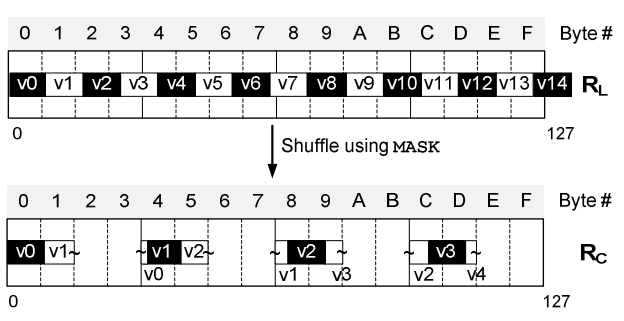
\includegraphics[width=\textwidth]{img/simd-align-1.png}
    \caption{...}
    \label{fig:simd-align-1} 
  \end{subfigure}
  \begin{subfigure}{0.45\textwidth}
    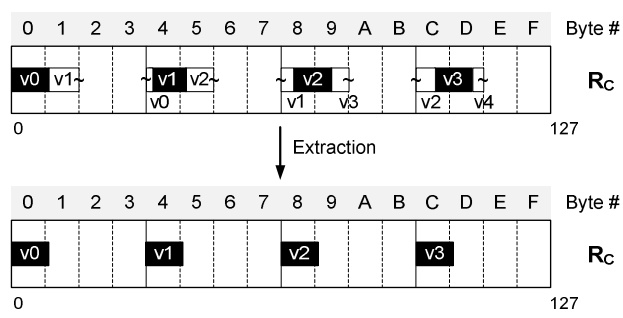
\includegraphics[width=\textwidth]{img/simd-align-2.png}
    \caption{...}
    \label{fig:simd-align-2} 
  \end{subfigure}
  \caption{Aligning a bitpacked vector for SIMD execution. Courtesy of \cite{Willhalm2009-hu}.}
  \label{fig:simd-align} 
\end{figure}
In order to use SIMD instructions, words must be aligned for the execution \cite{Willhalm2009-hu}, as seen in Figure \ref{fig:simd-align}.

Using its row-bank layout, \blink~has does not require aligning data in a word \cite{Johnson2008-cp}. For each partition, a special bitmap can be created to query the column. One or a couple of bitmap operations on every column, and then checking for null, predicates can be evaluated in a \textit{SIMD like fashion}.


\section{Scaling}
\label{sec:Scaling}
Scaling is necessary in large businesses, and volumes are increasing \cite{Qlik2012-ku}.

A system that supports this architecture can be scaled by adding more servers to the system cluster. We refer to this type of scaling as \textit{scaling out}. A system can also be scaled by adding more hardware, like more cores, more RAM, more powerful processors etc. to a single server. We refer to this type of scaling as \textit{scaling up}.

The best discussion on the need for scaling out can be found in research executed by Mukherjee \ea~\cite{Mukherjee2015-ul}. Historically, it has been argued that scaling out is the best way to acheive good performance. It does also provide redundancy; if one node in the cluster goes down, another node can be ready to take over.

However, there has been discussions that one should scale up instead of scale out. Wwhen using a shared-memory apporach, scaling up has been claimed to be easier \cite{Boncz2002-yj}. In addition, 80\% of Facebooks tasks is less than 10GB, a workload where a single server is sufficient \cite{Mukherjee2015-ul}. However, scaling up might also mean the transition to NUMA nodes, and these nodes (as we see in Section ?) benefit from software written for a distributed architecture. Last, but not least, if results are cached and used by several users, having one powerful server instead of several less powerful will increase cache hit rates \cite{qlik2012-ku}. \qlikview has reported that scaling up is twice as fast as scaling out on a large application with many users. For smaller applications, scaling up and scaling out gives the same performance.

Although \qlikview \cite{Qlik2012-ku} allows "proper" scaling out, that is distributing the work across multiple servers, single applications and data extracts can be spread across different servers. \todo{Elaborate and explain}



\section{Other}
\label{sec:Other}
Concurrency can be limited by having a maximum limit of concurrent queries. This is used in \ibm~\cite{Raman2013-em}.

None of this system investigated in this research have used the GPU for query processing. The reason for this might be because the GPU has bandwidth limitations \cite{Willhalm2009-hu} \todo{fill in}

The most trivial way to achieve better throughput is to allow multiple querys run at once. We refer to this technique as \textit{inter-query parallelism}.

For this to work well, query execution must be free for of locks, which is normally the case for read-only queries.

\section{Chapter Conclusion}
\label{sec:Chapter Conclusion}
We suggest using parallelization to utilize available CPU. 

We do not reccomend looking at scale-out yet, as this is harder to implement and degrades database cache performance. Instead, we recommend two scaling techniques:
\begin{itemize}
  \item Scale-out through spreading \bd~applications and data extracts across different servers.
  \item Scale-up by provisioning powerful, multicore CPUs and plenty of RAM.
\end{itemize}
